% Some commands used in this file
\newcommand{\package}{\emph}

\chapter{Introduction}
\label{chap:Introduction}

This chapter provides an easily accessible introduction to the subject covered by this thesis.  First, the main ingredients, namely Multipath TCP and SCION, are shortly introduced. Afterward, we explain how this work combines these two concepts with a shim, intermediary layer, and why this combination could be interesting. Every subject mentioned in this introduction is covered in more detail in the report's subsequent parts.

\section{Transmission Control Protocol (TCP)}

TCP stands for Transmission Control Protocol, a reliable, connection-oriented transport protocol in computer networks. It is one of the most important protocols and forms the basis of today's Internet. Connection-oriented means, that for every data transport between two entities, a fixed connection between the two endpoints is established. During all the data exchange, this fixed connection is then used, while none of the endpoints can influence the path the data takes through the network. As an example, imagine a user wants to surf its favorite web page: Upon starting browsing, TCP creates in the background a fixed connection between the user computer and the server hosting the page, illustrated in Figure \ref{fig:IntroTCP}. All data sent and received by the client's browser runs through this established connection.

\newpage

\begin{figure}[H]
	\begin{center}
		\def\svgwidth{1\textwidth}
		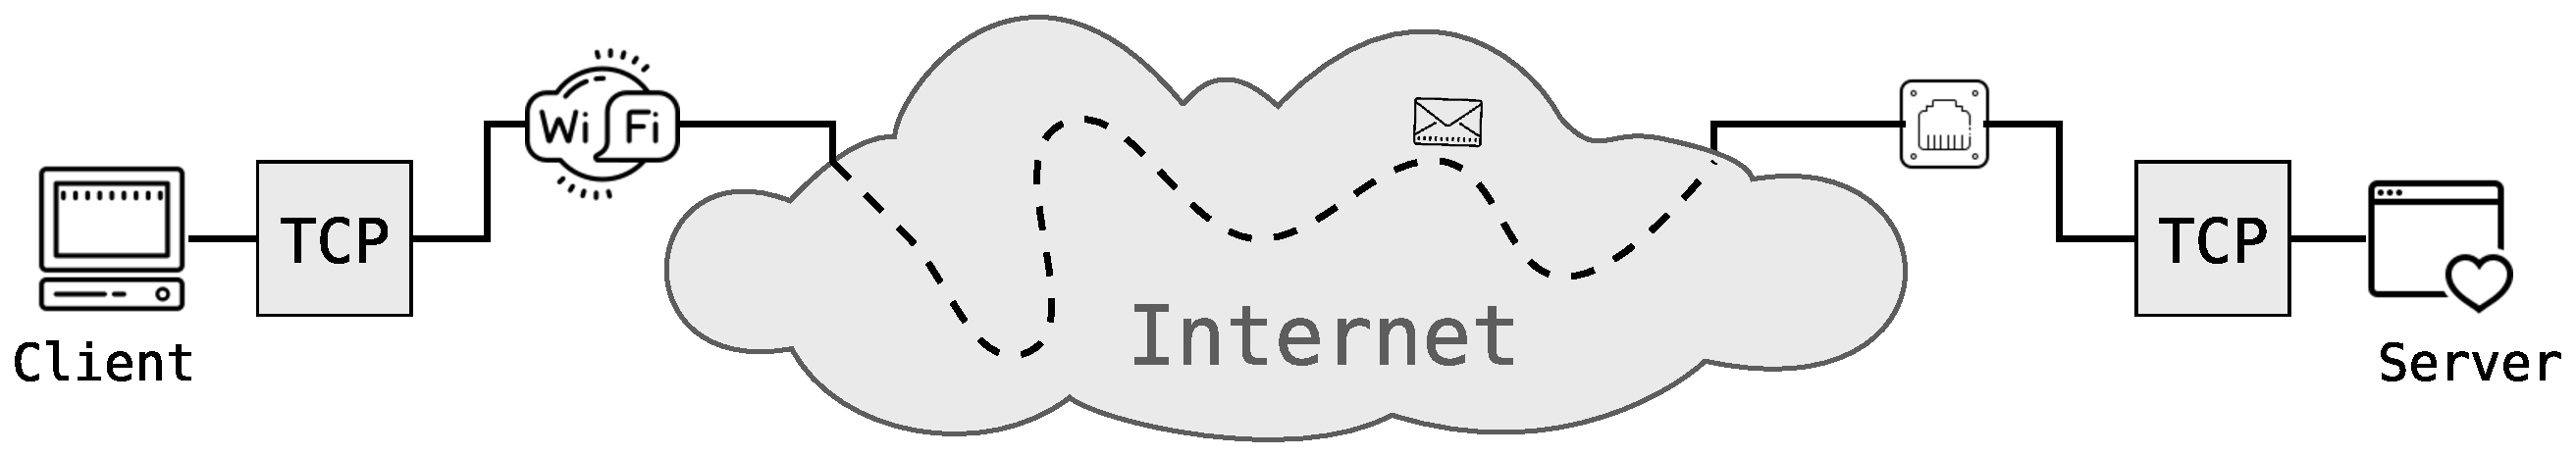
\includegraphics[scale=0.28]{../illustrations/introduction/TCPConnection.pdf}  
		\caption[Caption for the list of figures.]{Simplified illustration of TCP where the data exchange happens along a single fixed connection. The choice of the path taken cannot be influenced by the endpoints, in the illustration indicated by the dashed line.}
		\label{fig:IntroTCP}
	\end{center}
\end{figure}

\section{Multipath TCP (MPTCP)}

MPTCP stands for Multipath TCP and is an extension to TCP. It works exactly like TCP, with the only difference that all available network interfaces of a computer are used for the connection. This means that when the user visits his favorite website, MPTCP creates not just one connection, but one sub-connection, a so-called flow, for each interface available. Nowadays devices often have multiple attachment points to the Internet. So MPTCP creates, as illustrated in Figure \ref{fig:IntroMPTCP}, one flow via WLAN, one via cable and maybe even one via an analog dial-up modem. Thanks to these multiple flows, the protocol can improve reliability and performance. However, also with MPTCP, endpoints cannot influence what paths are taken by the individual flows. 

\begin{figure}[H]
	\begin{center}
		\def\svgwidth{1\textwidth}
		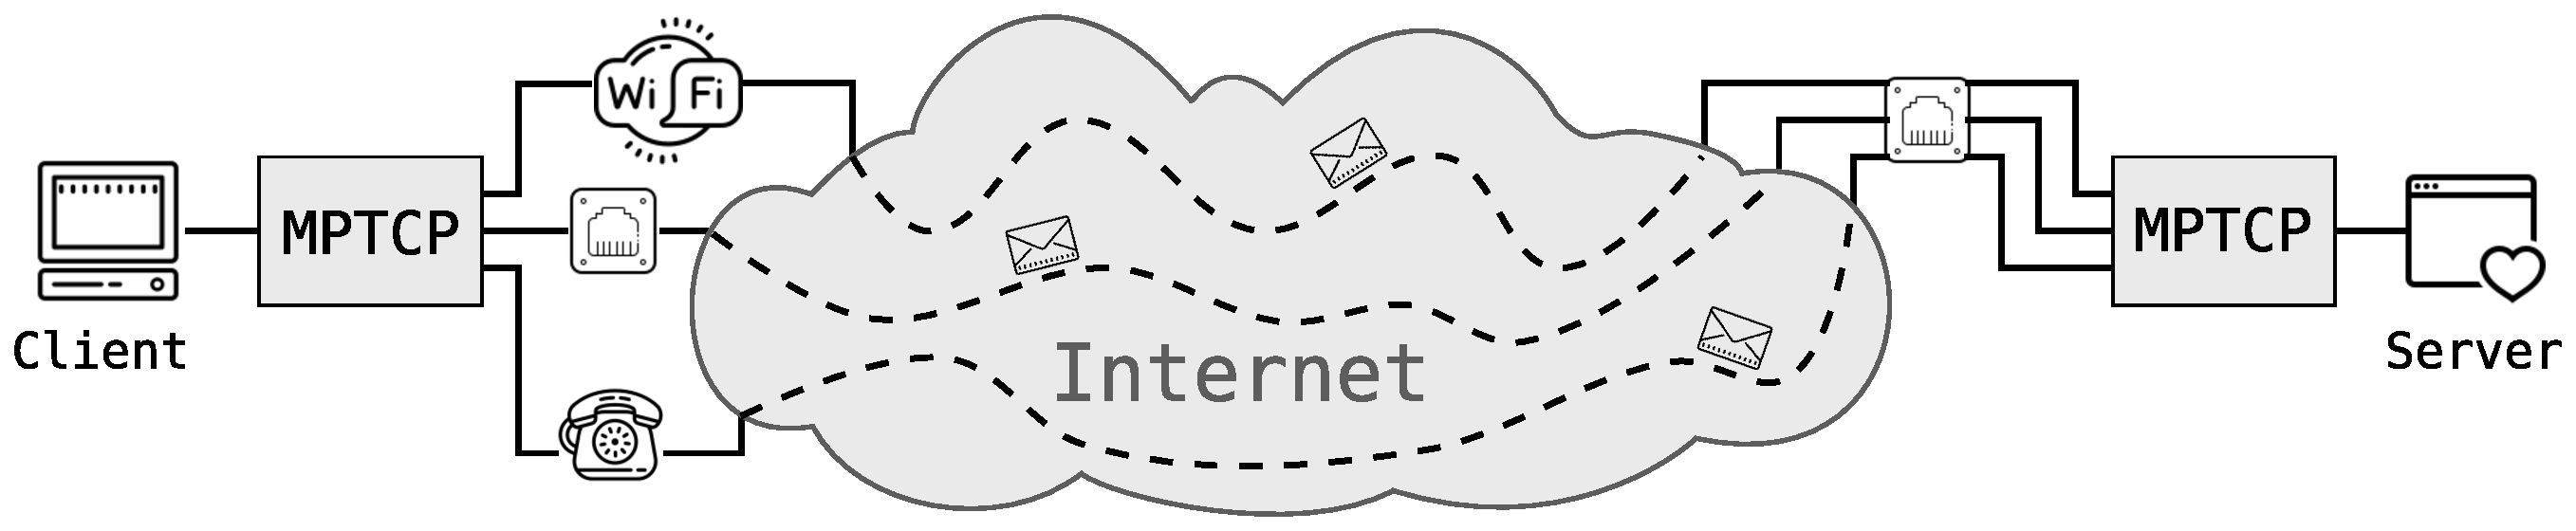
\includegraphics[scale=0.28]{../illustrations/introduction/MPTCPConnection.pdf}    
		\caption[Caption for the list of figures.]{Simplified illustration of MPTCP, where the endpoints use all available network interfaces for the data exchange. As for TCP, the choice for the paths taken cannot be influenced by the user.}
		\label{fig:IntroMPTCP}
	\end{center}
\end{figure}

\section{SCION}

Scalability, Control and Isolation on next-generation Networks or SCION for short is a new type of internet architecture, which has been developed by ETH Zurich for several years. SCION re-implements existing Internet protocols taking known vulnerabilities into account. It is more resource-efficient and reduces the supremacy of individual actors through its decentralized infrastructure. An important feature of the architecture, illustrated in Figure \ref{fig:IntroSCION}, is that endpoints can determine the path taken by its data through the network. Senders can choose the path along which they want to send their data, receivers can choose from which paths they want to receive data.

\begin{figure}[H]
	\begin{center}
		\def\svgwidth{1\textwidth}
		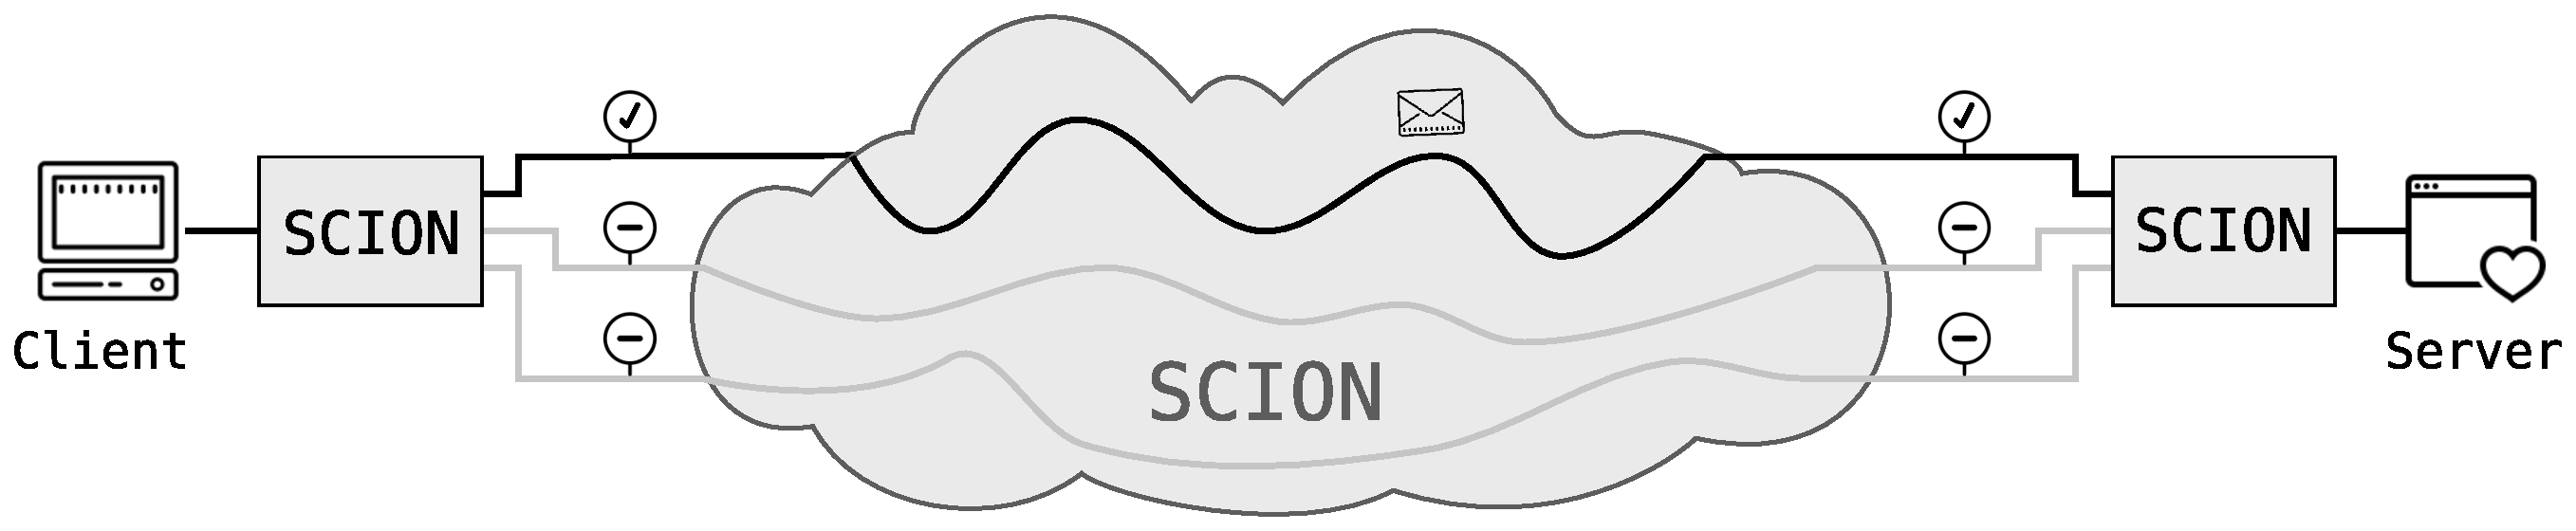
\includegraphics[scale=0.28]{../illustrations/introduction/SCION.pdf}
		\caption[Caption for the list of figures.]{Simplified illustration of the SCION internet architecture where the endpoints can determine which paths their data takes through the network.}
		\label{fig:IntroSCION}
	\end{center}
\end{figure}

\section{Shila}

\subsection*{Functionality}

Shila is the abbreviation for Shim Layer and is the main contribution of this work. It acts as a mediating layer and enables the use of MPTCP in the SCION internet architecture; illustrated in Figure \ref{fig:IntroRoleOfShila}. 

\begin{figure}[H]
	\begin{center}
		\def\svgwidth{1\textwidth}
		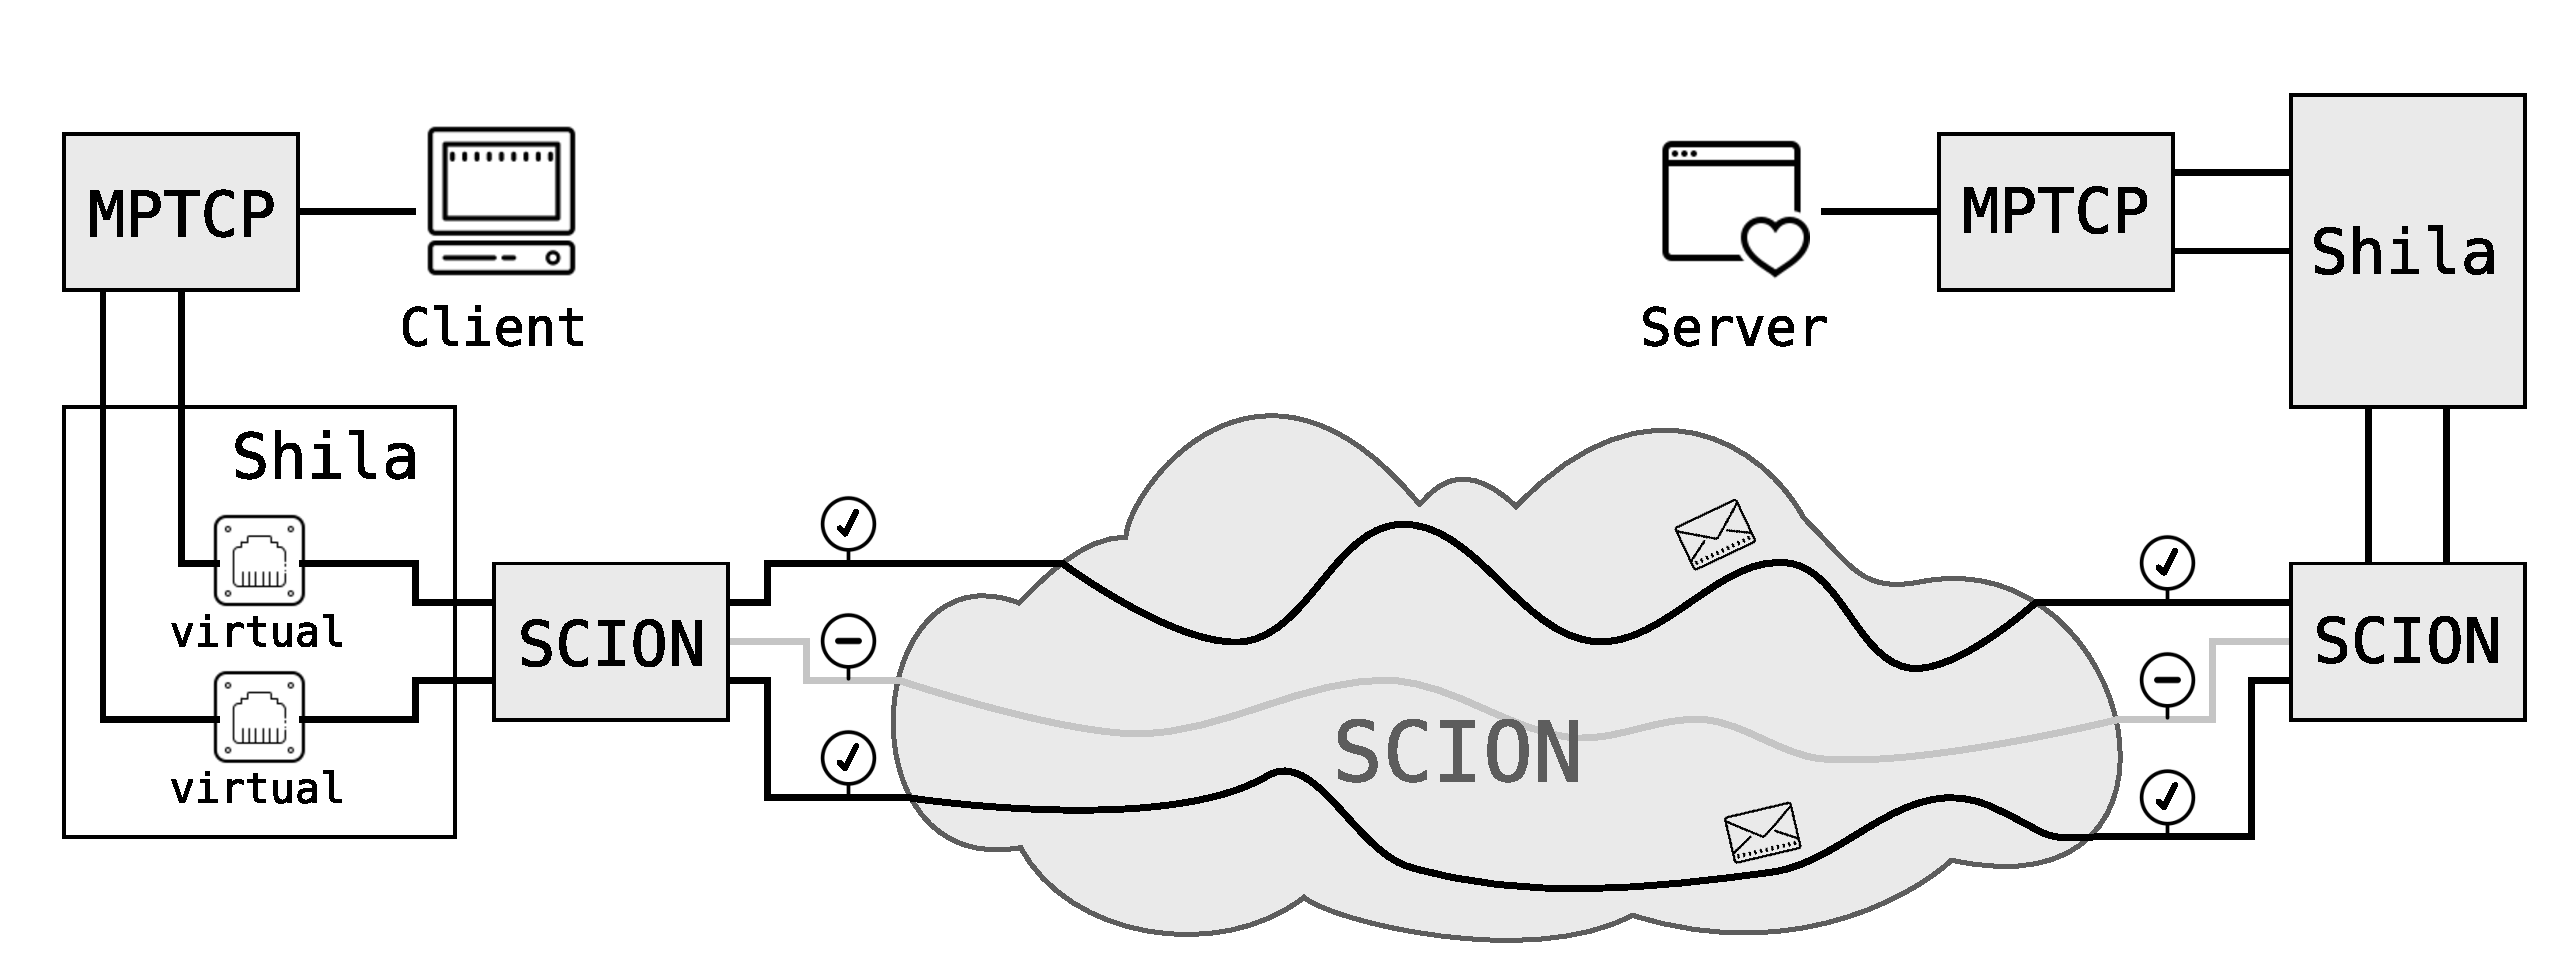
\includegraphics[scale=0.28]{../illustrations/introduction/Shila.pdf} 
		\caption[Caption for the list of figures.]{Simplified illustration of the functionality of Shila: It acts as an intermediate layer between MPTCP and SCION, provides virtual interfaces to MPTCP and redirects the intercepted flows through the SCION network.}
		\label{fig:IntroRoleOfShila}
	\end{center}
\end{figure}

Upon startup, Shila creates and monitors a user-selectable number of virtual network interfaces. A virtual interface is a fake connection to a network, which is perceived by the computer as a real one. If now someone visits his favorite homepage, Multipath TCP tries to connect to the server via these virtual interfaces. Shila detects this connection establishment and redirects the data flow.  For every flow created by MPTCP, the Shila instance creates a connection over SCION to the Shila instance running on the server and forwards the respective data traffic. The shim layer on the server side receives the data and distributes it through the MPTCP functionality to the server application.

\subsection*{Benefit}

The new internet architecture SCION offers great advantages over the existing Internet in terms of security and reliability. However, the transfer from such an established infrastructure as the current Internet to new technology is a big challenge. Applications rely on established programming interfaces and protocols and are programmed accordingly. A re-implementation of all software so that it can be used in a new architecture seems utopian. For the deployment of SCION, it is therefore of great importance that existing applications can be used in the new network with as little effort as possible. The implementation of Shila enables exactly this. All applications that use TCP for their communications can be operated via SCION without the need for internal changes. With Shila, your favorite TCP application can be run over SCION without much effort - a good reason to try the new infrastructure.

If the endpoints furthermore support MPTCP, the application can additionally benefit from the advantages of the multipath protocol and the support of multiple paths in SCION. But not only that, with Shila in its mediating role in between, there is further potential. To give a possible example, let's look at the use of MPTCP in today's Internet. It is quite possible that several flows of an MPTCP connection use the same link for certain parts of the path on the Internet. In order not to disadvantage other users, a fairness algorithm\footnote{Ensuring fairness is part of Congestion Control. However, to keep the introduction as generally understandable as possible, we don't use this term here.} monitors and controls the use of bandwidth. This is to ensure that all flows of an MPTCP connection going through the same link do not have more bandwidth available than the connection of another user. As we have seen, the endpoints on the Internet today are unaware of the paths their data takes. The same applies to the fairness algorithm, it has also no idea what paths are taken and can therefore not tell whether shared sub-paths exist or not. It has to act conservatively. If we use Shila to run our applications with MPTCP over the SCION network, Shila could ensure that no links are shared when choosing the paths of the individual flows. This makes it possible to disable the fairness algorithm or at least make it less strict, which results in better performance of the data transfer.